%% bare_adv.tex
%% V1.4b
%% 2015/08/26
%% by Michael Shell
%% See: 
%% http://www.michaelshell.org/
%% for current contact information.
%%
%% This is a skeleton file demonstrating the advanced use of IEEEtran.cls
%% (requires IEEEtran.cls version 1.8b or later) with an IEEE Computer
%% Society journal paper.
%%
%% Support sites:
%% http://www.michaelshell.org/tex/ieeetran/
%% http://www.ctan.org/pkg/ieeetran
%% and
%% http://www.ieee.org/

%%*************************************************************************
%% Legal Notice:
%% This code is offered as-is without any warranty either expressed or
%% implied; without even the implied warranty of MERCHANTABILITY or
%% FITNESS FOR A PARTICULAR PURPOSE! 
%% User assumes all risk.
%% In no event shall the IEEE or any contributor to this code be liable for
%% any damages or losses, including, but not limited to, incidental,
%% consequential, or any other damages, resulting from the use or misuse
%% of any information contained here.
%%
%% All comments are the opinions of their respective authors and are not
%% necessarily endorsed by the IEEE.
%%
%% This work is distributed under the LaTeX Project Public License (LPPL)
%% ( http://www.latex-project.org/ ) version 1.3, and may be freely used,
%% distributed and modified. A copy of the LPPL, version 1.3, is included
%% in the base LaTeX documentation of all distributions of LaTeX released
%% 2003/12/01 or later.
%% Retain all contribution notices and credits.
%% ** Modified files should be clearly indicated as such, including  **
%% ** renaming them and changing author support contact information. **
%%*************************************************************************


% *** Authors should verify (and, if needed, correct) their LaTeX system  ***
% *** with the testflow diagnostic prior to trusting their LaTeX platform ***
% *** with production work. The IEEE's font choices and paper sizes can   ***
% *** trigger bugs that do not appear when using other class files.       ***                          ***
% The testflow support page is at:
% http://www.michaelshell.org/tex/testflow/


% IEEEtran V1.7 and later provides for these CLASSINPUT macros to allow the
% user to reprogram some IEEEtran.cls defaults if needed. These settings
% override the internal defaults of IEEEtran.cls regardless of which class
% options are used. Do not use these unless you have good reason to do so as
% they can result in nonIEEE compliant documents. User beware. ;)
%
%\newcommand{\CLASSINPUTbaselinestretch}{1.0} % baselinestretch
%\newcommand{\CLASSINPUTinnersidemargin}{1in} % inner side margin
%\newcommand{\CLASSINPUToutersidemargin}{1in} % outer side margin
%\newcommand{\CLASSINPUTtoptextmargin}{1in}   % top text margin
%\newcommand{\CLASSINPUTbottomtextmargin}{1in}% bottom text margin




%
\documentclass[10pt,journal,compsoc]{IEEEtran}
\usepackage{CTEX}
\usepackage{diagbox}
\usepackage[justification=centering]{caption}
% If IEEEtran.cls has not been installed into the LaTeX system files,
% manually specify the path to it like:
% \documentclass[10pt,journal,compsoc]{../sty/IEEEtran}


% For Computer Society journals, IEEEtran defaults to the use of 
% Palatino/Palladio as is done in IEEE Computer Society journals.
% To go back to Times Roman, you can use this code:
%\renewcommand{\rmdefault}{ptm}\selectfont





% Some very useful LaTeX packages include:
% (uncomment the ones you want to load)



% *** MISC UTILITY PACKAGES ***
%
%\usepackage{ifpdf}
% Heiko Oberdiek's ifpdf.sty is very useful if you need conditional
% compilation based on whether the output is pdf or dvi.
% usage:
% \ifpdf
%   % pdf code
% \else
%   % dvi code
% \fi
% The latest version of ifpdf.sty can be obtained from:
% http://www.ctan.org/pkg/ifpdf
% Also, note that IEEEtran.cls V1.7 and later provides a builtin
% \ifCLASSINFOpdf conditional that works the same way.
% When switching from latex to pdflatex and vice-versa, the compiler may
% have to be run twice to clear warning/error messages.




% *** CITATION PACKAGES ***
%
\ifCLASSOPTIONcompsoc
  % The IEEE Computer Society needs nocompress option
  % requires cite.sty v4.0 or later (November 2003)
  \usepackage[nocompress]{cite}
\else
  % normal IEEE
  \usepackage{cite}
\fi
% cite.sty was written by Donald Arseneau
% V1.6 and later of IEEEtran pre-defines the format of the cite.sty package
% \cite{} output to follow that of the IEEE. Loading the cite package will
% result in citation numbers being automatically sorted and properly
% "compressed/ranged". e.g., \cite{ShiZhongci2000}, \cite{QiuXipeng2020}, \cite{LuJinfu2004}, \cite{duraisamy2015}, \cite{kopriva2009}, \cite{wang2017} without using
% cite.sty will become \cite{ShiZhongci2000}, \cite{LuJinfu2004}, \cite{kopriva2009}--\cite{duraisamy2015}, \cite{QiuXipeng2020} using cite.sty. cite.sty's
% \cite will automatically add leading space, if needed. Use cite.sty's
% noadjust option (cite.sty V3.8 and later) if you want to turn this off
% such as if a citation ever needs to be enclosed in parenthesis.
% cite.sty is already installed on most LaTeX systems. Be sure and use
% version 5.0 (2009-03-20) and later if using hyperref.sty.
% The latest version can be obtained at:
% http://www.ctan.org/pkg/cite
% The documentation is contained in the cite.sty file itself.
%
% Note that some packages require special options to format as the Computer
% Society requires. In particular, Computer Society  papers do not use
% compressed citation ranges as is done in typical IEEE papers
% (e.g., \cite{ShiZhongci2000}-\cite{chapra1998}). Instead, they list every citation separately in order
% (e.g., \cite{ShiZhongci2000}, \cite{LuJinfu2004}, \cite{logan2014}, \cite{chapra1998}). To get the latter we need to load the cite
% package with the nocompress option which is supported by cite.sty v4.0
% and later.



\usepackage{graphics}

% *** GRAPHICS RELATED PACKAGES ***
%
\ifCLASSINFOpdf
   \usepackage[pdftex]{graphicx}
  % declare the path(s) where your graphic files are
  % \graphicspath{{../pdf/}{../jpeg/}}
  % and their extensions so you won't have to specify these with
  % every instance of \includegraphics
  % \DeclareGraphicsExtensions{.pdf,.jpeg,.png}
\else
  % or other class option (dvipsone, dvipdf, if not using dvips). graphicx
  % will default to the driver specified in the system graphics.cfg if no
  % driver is specified.
  \usepackage[dvips]{graphicx}
  % declare the path(s) where your graphic files are
  % \graphicspath{{../eps/}}
  % and their extensions so you won't have to specify these with
  % every instance of \includegraphics
  % \DeclareGraphicsExtensions{.eps}
\fi
% graphicx was written by David Carlisle and Sebastian Rahtz. It is
% required if you want graphics, photos, etc. graphicx.sty is already
% installed on most LaTeX systems. The latest version and documentation
% can be obtained at: 
% http://www.ctan.org/pkg/graphicx
% Another good source of documentation is "Using Imported Graphics in
% LaTeX2e" by Keith Reckdahl which can be found at:
% http://www.ctan.org/pkg/epslatex
%
% latex, and pdflatex in dvi mode, support graphics in encapsulated
% postscript (.eps) format. pdflatex in pdf mode supports graphics
% in .pdf, .jpeg, .png and .mps (metapost) formats. Users should ensure
% that all non-photo figures use a vector format (.eps, .pdf, .mps) and
% not a bitmapped formats (.jpeg, .png). The IEEE frowns on bitmapped formats
% which can result in "jaggedy"/blurry rendering of lines and letters as
% well as large increases in file sizes.
%
% You can find documentation about the pdfTeX application at:
% http://www.tug.org/applications/pdftex





% *** MATH PACKAGES ***

\usepackage{amsmath}
\usepackage{amssymb}
% A popular package from the American Mathematical Society that provides
% many useful and powerful commands for dealing with mathematics.
%
% Note that the amsmath package sets \interdisplaylinepenalty to 10000
% thus preventing page breaks from occurring within multiline equations. Use:
%\interdisplaylinepenalty=2500
% after loading amsmath to restore such page breaks as IEEEtran.cls normally
% does. amsmath.sty is already installed on most LaTeX systems. The latest
% version and documentation can be obtained at:
% http://www.ctan.org/pkg/amsmath





% *** SPECIALIZED LIST PACKAGES ***
%\usepackage{acronym}
% acronym.sty was written by Tobias Oetiker. This package provides tools for
% managing documents with large numbers of acronyms. (You don't *have* to
% use this package - unless you have a lot of acronyms, you may feel that
% such package management of them is bit of an overkill.)
% Do note that the acronym environment (which lists acronyms) will have a
% problem when used under IEEEtran.cls because acronym.sty relies on the
% description list environment - which IEEEtran.cls has customized for
% producing IEEE style lists. A workaround is to declared the longest
% label width via the IEEEtran.cls \IEEEiedlistdecl global control:
%
% \renewcommand{\IEEEiedlistdecl}{\IEEEsetlabelwidth{SONET}}
% \begin{acronym}
%
% \end{acronym}
% \renewcommand{\IEEEiedlistdecl}{\relax}% remember to reset \IEEEiedlistdecl
%
% instead of using the acronym environment's optional argument.
% The latest version and documentation can be obtained at:
% http://www.ctan.org/pkg/acronym


\usepackage{algorithmic}
% algorithmic.sty was written by Peter Williams and Rogerio Brito.
% This package provides an algorithmic environment fo describing algorithms.
% You can use the algorithmic environment in-text or within a figure
% environment to provide for a floating algorithm. Do NOT use the algorithm
% floating environment provided by algorithm.sty (by the same authors) or
% algorithm2e.sty (by Christophe Fiorio) as the IEEE does not use dedicated
% algorithm float types and packages that provide these will not provide
% correct IEEE style captions. The latest version and documentation of
% algorithmic.sty can be obtained at:
% http://www.ctan.org/pkg/algorithms
% Also of interest may be the (relatively newer and more customizable)
% algorithmicx.sty package by Szasz Janos:
% http://www.ctan.org/pkg/algorithmicx




% *** ALIGNMENT PACKAGES ***
%
\usepackage{array}
% Frank Mittelbach's and David Carlisle's array.sty patches and improves
% the standard LaTeX2e array and tabular environments to provide better
% appearance and additional user controls. As the default LaTeX2e table
% generation code is lacking to the point of almost being broken with
% respect to the quality of the end results, all users are strongly
% advised to use an enhanced (at the very least that provided by array.sty)
% set of table tools. array.sty is already installed on most systems. The
% latest version and documentation can be obtained at:
% http://www.ctan.org/pkg/array


%\usepackage{mdwmath}
%\usepackage{mdwtab}
% Also highly recommended is Mark Wooding's extremely powerful MDW tools,
% especially mdwmath.sty and mdwtab.sty which are used to format equations
% and tables, respectively. The MDWtools set is already installed on most
% LaTeX systems. The lastest version and documentation is available at:
% http://www.ctan.org/pkg/mdwtools


% IEEEtran contains the IEEEeqnarray family of commands that can be used to
% generate multiline equations as well as matrices, tables, etc., of high
% quality.


%\usepackage{eqparbox}
% Also of notable interest is Scott Pakin's eqparbox package for creating
% (automatically sized) equal width boxes - aka "natural width parboxes".
% Available at:
% http://www.ctan.org/pkg/eqparbox




% *** SUBFIGURE PACKAGES ***

\usepackage[caption=false,font=footnotesize]{subfig}

% subfig.sty, written by Steven Douglas Cochran, is the modern replacement
% for subfigure.sty, the latter of which is no longer maintained and is
% incompatible with some LaTeX packages including fixltx2e. However,
% subfig.sty requires and automatically loads Axel Sommerfeldt's caption.sty
% which will override IEEEtran.cls' handling of captions and this will result
% in non-IEEE style figure/table captions. To prevent this problem, be sure
% and invoke subfig.sty's "caption=false" package option (available since
% subfig.sty version 1.3, 2005/06/28) as this is will preserve IEEEtran.cls
% handling of captions.
% Note that the Computer Society format requires a sans serif font rather
% than the serif font used in traditional IEEE formatting and thus the need
% to invoke different subfig.sty package options depending on whether
% compsoc mode has been enabled.
%
% The latest version and documentation of subfig.sty can be obtained at:
% http://www.ctan.org/pkg/subfig




% *** FLOAT PACKAGES ***
%
%\usepackage{fixltx2e}
% fixltx2e, the successor to the earlier fix2col.sty, was written by
% Frank Mittelbach and David Carlisle. This package corrects a few problems
% in the LaTeX2e kernel, the most notable of which is that in current
% LaTeX2e releases, the ordering of single and double column floats is not
% guaranteed to be preserved. Thus, an unpatched LaTeX2e can allow a
% single column figure to be placed prior to an earlier double column
% figure.
% Be aware that LaTeX2e kernels dated 2015 and later have fixltx2e.sty's
% corrections already built into the system in which case a warning will
% be issued if an attempt is made to load fixltx2e.sty as it is no longer
% needed.
% The latest version and documentation can be found at:
% http://www.ctan.org/pkg/fixltx2e


%\usepackage{stfloats}
% stfloats.sty was written by Sigitas Tolusis. This package gives LaTeX2e
% the ability to do double column floats at the bottom of the page as well
% as the top. (e.g., "\begin{figure*}[!b]" is not normally possible in
% LaTeX2e). It also provides a command:
%\fnbelowfloat
% to enable the placement of footnotes below bottom floats (the standard
% LaTeX2e kernel puts them above bottom floats). This is an invasive package
% which rewrites many portions of the LaTeX2e float routines. It may not work
% with other packages that modify the LaTeX2e float routines. The latest
% version and documentation can be obtained at:
% http://www.ctan.org/pkg/stfloats
% Do not use the stfloats baselinefloat ability as the IEEE does not allow
% \baselineskip to stretch. Authors submitting work to the IEEE should note
% that the IEEE rarely uses double column equations and that authors should try
% to avoid such use. Do not be tempted to use the cuted.sty or midfloat.sty
% packages (also by Sigitas Tolusis) as the IEEE does not format its papers in
% such ways.
% Do not attempt to use stfloats with fixltx2e as they are incompatible.
% Instead, use Morten Hogholm'a dblfloatfix which combines the features
% of both fixltx2e and stfloats:
%
% \usepackage{dblfloatfix}
% The latest version can be found at:
% http://www.ctan.org/pkg/dblfloatfix


%\ifCLASSOPTIONcaptionsoff
%  \usepackage[nomarkers]{endfloat}
% \let\MYoriglatexcaption\caption
% \renewcommand{\caption}\cite{LuJinfu2004}[\relax]{\MYoriglatexcaption[#2]{#2}}
%\fi
% endfloat.sty was written by James Darrell McCauley, Jeff Goldberg and 
% Axel Sommerfeldt. This package may be useful when used in conjunction with 
% IEEEtran.cls'  captionsoff option. Some IEEE journals/societies require that
% submissions have lists of figures/tables at the end of the paper and that
% figures/tables without any captions are placed on a page by themselves at
% the end of the document. If needed, the draftcls IEEEtran class option or
% \CLASSINPUTbaselinestretch interface can be used to increase the line
% spacing as well. Be sure and use the nomarkers option of endfloat to
% prevent endfloat from "marking" where the figures would have been placed
% in the text. The two hack lines of code above are a slight modification of
% that suggested by in the endfloat docs (section 8.4.1) to ensure that
% the full captions always appear in the list of figures/tables - even if
% the user used the short optional argument of \caption[]{}.
% IEEE papers do not typically make use of \caption[]'s optional argument,
% so this should not be an issue. A similar trick can be used to disable
% captions of packages such as subfig.sty that lack options to turn off
% the subcaptions:
% For subfig.sty:
% \let\MYorigsubfloat\subfloat
% \renewcommand{\subfloat}\cite{LuJinfu2004}[\relax]{\MYorigsubfloat[]{#2}}
% However, the above trick will not work if both optional arguments of
% the \subfloat command are used. Furthermore, there needs to be a
% description of each subfigure *somewhere* and endfloat does not add
% subfigure captions to its list of figures. Thus, the best approach is to
% avoid the use of subfigure captions (many IEEE journals avoid them anyway)
% and instead reference/explain all the subfigures within the main caption.
% The latest version of endfloat.sty and its documentation can obtained at:
% http://www.ctan.org/pkg/endfloat
%
% The IEEEtran \ifCLASSOPTIONcaptionsoff conditional can also be used
% later in the document, say, to conditionally put the References on a 
% page by themselves.





% *** PDF, URL AND HYPERLINK PACKAGES ***
%
\usepackage{url}
% url.sty was written by Donald Arseneau. It provides better support for
% handling and breaking URLs. url.sty is already installed on most LaTeX
% systems. The latest version and documentation can be obtained at:
% http://www.ctan.org/pkg/url
% Basically, \url{my_url_here}.


% NOTE: PDF thumbnail features are not required in IEEE papers
%       and their use requires extra complexity and work.
%\ifCLASSINFOpdf
%  \usepackage[pdftex]{thumbpdf}
%\else
%  \usepackage[dvips]{thumbpdf}
%\fi
% thumbpdf.sty and its companion Perl utility were written by Heiko Oberdiek.
% It allows the user a way to produce PDF documents that contain fancy
% thumbnail images of each of the pages (which tools like acrobat reader can
% utilize). This is possible even when using dvi->ps->pdf workflow if the
% correct thumbpdf driver options are used. thumbpdf.sty incorporates the
% file containing the PDF thumbnail information (filename.tpm is used with
% dvips, filename.tpt is used with pdftex, where filename is the base name of
% your tex document) into the final ps or pdf output document. An external
% utility, the thumbpdf *Perl script* is needed to make these .tpm or .tpt
% thumbnail files from a .ps or .pdf version of the document (which obviously
% does not yet contain pdf thumbnails). Thus, one does a:
% 
% thumbpdf filename.pdf 
%
% to make a filename.tpt, and:
%
% thumbpdf --mode dvips filename.ps
%
% to make a filename.tpm which will then be loaded into the document by
% thumbpdf.sty the NEXT time the document is compiled (by pdflatex or
% latex->dvips->ps2pdf). Users must be careful to regenerate the .tpt and/or
% .tpm files if the main document changes and then to recompile the
% document to incorporate the revised thumbnails to ensure that thumbnails
% match the actual pages. It is easy to forget to do this!
% 
% Unix systems come with a Perl interpreter. However, MS Windows users
% will usually have to install a Perl interpreter so that the thumbpdf
% script can be run. The Ghostscript PS/PDF interpreter is also required.
% See the thumbpdf docs for details. The latest version and documentation
% can be obtained at.
% http://www.ctan.org/pkg/thumbpdf


% NOTE: PDF hyperlink and bookmark features are not required in IEEE
%       papers and their use requires extra complexity and work.
% *** IF USING HYPERREF BE SURE AND CHANGE THE EXAMPLE PDF ***
% *** TITLE/SUBJECT/AUTHOR/KEYWORDS INFO BELOW!!           ***
\newcommand\MYhyperrefoptions{bookmarks=true,bookmarksnumbered=true,
pdfpagemode={UseOutlines},plainpages=false,pdfpagelabels=true,
colorlinks=true,linkcolor={black},citecolor={black},urlcolor={black},
pdftitle={Bare Demo of IEEEtran.cls for Computer Society Journals},%<!CHANGE!
pdfsubject={Typesetting},%<!CHANGE!
pdfauthor={Michael D. Shell},%<!CHANGE!
pdfkeywords={Computer Society, IEEEtran, journal, LaTeX, paper,
             template}}%<^!CHANGE!
%\ifCLASSINFOpdf
%\usepackage[\MYhyperrefoptions,pdftex]{hyperref}
%\else
%\usepackage[\MYhyperrefoptions,breaklinks=true,dvips]{hyperref}
%\usepackage{breakurl}
%\fi
% One significant drawback of using hyperref under DVI output is that the
% LaTeX compiler cannot break URLs across lines or pages as can be done
% under pdfLaTeX's PDF output via the hyperref pdftex driver. This is
% probably the single most important capability distinction between the
% DVI and PDF output. Perhaps surprisingly, all the other PDF features
% (PDF bookmarks, thumbnails, etc.) can be preserved in
% .tex->.dvi->.ps->.pdf workflow if the respective packages/scripts are
% loaded/invoked with the correct driver options (dvips, etc.). 
% As most IEEE papers use URLs sparingly (mainly in the references), this
% may not be as big an issue as with other publications.
%
% That said, Vilar Camara Neto created his breakurl.sty package which
% permits hyperref to easily break URLs even in dvi mode.
% Note that breakurl, unlike most other packages, must be loaded
% AFTER hyperref. The latest version of breakurl and its documentation can
% be obtained at:
% http://www.ctan.org/pkg/breakurl
% breakurl.sty is not for use under pdflatex pdf mode.
%
% The advanced features offer by hyperref.sty are not required for IEEE
% submission, so users should weigh these features against the added
% complexity of use.
% The package options above demonstrate how to enable PDF bookmarks
% (a type of table of contents viewable in Acrobat Reader) as well as
% PDF document information (title, subject, author and keywords) that is
% viewable in Acrobat reader's Document_Properties menu. PDF document
% information is also used extensively to automate the cataloging of PDF
% documents. The above set of options ensures that hyperlinks will not be
% colored in the text and thus will not be visible in the printed page,
% but will be active on "mouse over". USING COLORS OR OTHER HIGHLIGHTING
% OF HYPERLINKS CAN RESULT IN DOCUMENT REJECTION BY THE IEEE, especially if
% these appear on the "printed" page. IF IN DOUBT, ASK THE RELEVANT
% SUBMISSION EDITOR. You may need to add the option hypertexnames=false if
% you used duplicate equation numbers, etc., but this should not be needed
% in normal IEEE work.
% The latest version of hyperref and its documentation can be obtained at:
% http://www.ctan.org/pkg/hyperref





% *** Do not adjust lengths that control margins, column widths, etc. ***
% *** Do not use packages that alter fonts (such as pslatex).         ***
% There should be no need to do such things with IEEEtran.cls V1.6 and later.
% (Unless specifically asked to do so by the journal or conference you plan
% to submit to, of course. )


% correct bad hyphenation here
\hyphenation{op-tical net-works semi-conduc-tor}


\begin{document}
%
% paper title
% Titles are generally capitalized except for words such as a, an, and, as,
% at, but, by, for, in, nor, of, on, or, the, to and up, which are usually
% not capitalized unless they are the first or last word of the title.
% Linebreaks \\ can be used within to get better formatting as desired.
% Do not put math or special symbols in the title.
\title{缓存替换策略综述}
%
%
% author names and IEEE memberships
% note positions of commas and nonbreaking spaces ( ~ ) LaTeX will not break
% a structure at a ~ so this keeps an author's name from being broken across
% two lines.
% use \thanks{} to gain access to the first footnote area
% a separate \thanks must be used for each paragraph as LaTeX2e's \thanks
% was not built to handle multiple paragraphs
%
%
%\IEEEcompsocitemizethanks is a special \thanks that produces the bulleted
% lists the Computer Society journals use for "first footnote" author
% affiliations. Use \IEEEcompsocthanksitem which works much like \item
% for each affiliation group. When not in compsoc mode,
% \IEEEcompsocitemizethanks becomes like \thanks and
% \IEEEcompsocthanksitem becomes a line break with idention. This
% facilitates dual compilation, although admittedly the differences in the
% desired content of \author between the different types of papers makes a
% one-size-fits-all approach a daunting prospect. For instance, compsoc 
% journal papers have the author affiliations above the "Manuscript
% received ..."  text while in non-compsoc journals this is reversed. Sigh.

\author{史鸿儒 \\
\IEEEmembership{(22235086,浙江大学数学科学学院)} 
}

% note the % following the last \IEEEmembership and also \thanks - 
% these prevent an unwanted space from occurring between the last author name
% and the end of the author line. i.e., if you had this:
% 
% \author{....lastname \thanks{...} \thanks{...} }
%                     ^------------^------------^----Do not want these spaces!
%
% a space would be appended to the last name and could cause every name on that
% line to be shifted left slightly. This is one of those "LaTeX things". For
% instance, "\textbf{A} \textbf{B}" will typeset as "A B" not "AB". To get
% "AB" then you have to do: "\textbf{A}\textbf{B}"
% \thanks is no different in this regard, so shield the last } of each \thanks
% that ends a line with a % and do not let a space in before the next \thanks.
% Spaces after \IEEEmembership other than the last one are OK (and needed) as
% you are supposed to have spaces between the names. For what it is worth,
% this is a minor point as most people would not even notice if the said evil
% space somehow managed to creep in.



% The paper headers
\markboth{Hongru Shi, 22235086}%
{Shell \MakeLowercase{\textit{et al.}}: Bare Advanced Demo of IEEEtran.cls for IEEE Computer Society Journals}
% The only time the second header will appear is for the odd numbered pages
% after the title page when using the twoside option.
% 
% *** Note that you probably will NOT want to include the author's ***
% *** name in the headers of peer review papers.                   ***
% You can use \ifCLASSOPTIONpeerreview for conditional compilation here if
% you desire.



% The publisher's ID mark at the bottom of the page is less important with
% Computer Society journal papers as those publications place the marks
% outside of the main text columns and, therefore, unlike regular IEEE
% journals, the available text space is not reduced by their presence.
% If you want to put a publisher's ID mark on the page you can do it like
% this:
%\IEEEpubid{0000--0000/00\$00.00~\copyright~2015 IEEE}
% or like this to get the Computer Society new two part style.
%\IEEEpubid{\makebox[\columnwidth]{\hfill 0000--0000/00/\$00.00~\copyright~2015 IEEE}%
%\hspace{\columnsep}\makebox[\columnwidth]{Published by the IEEE Computer Society\hfill}}
% Remember, if you use this you must call \IEEEpubidadjcol in the second
% column for its text to clear the IEEEpubid mark (Computer Society journal
% papers don't need this extra clearance.)



% use for special paper notices
%\IEEEspecialpapernotice{(Invited Paper)}



% for Computer Society papers, we must declare the abstract and index terms
% PRIOR to the title within the \IEEEtitleabstractindextext IEEEtran
% command as these need to go into the title area created by \maketitle.
% As a general rule, do not put math, special symbols or citations
% in the abstract or keywords.
\IEEEtitleabstractindextext{%
\begin{abstract}
高速缓存是现代处理器中的重要组件。缓存的有效性在很大程度上受其替换策略的影响。本文中我们主要介绍四种缓存替换策略,它们是在一些经典的缓存替换策略的基础上,进行改进。第一个是P-OPT,这是一个应用在图处理方面的缓存替换策略。第二个是Ripple,这是一种完全基于软件的策略,能够优化硬件上的替换策略,并且是一种指令缓存替换策略。第三种是RLR,这是利用强化学习推导出了一个新的缓存替换策略强化学习替换策略(Replacment Learned Replacement)。第四种是Glider,这种替换策略建立在 Hawkeye 缓存替换策略的基础上,利用深度学习推导。
\end{abstract}

% Note that keywords are not normally used for peerreview papers.
\begin{IEEEkeywords}
缓存替换,P-OPT,Ripple,RLR,Glider。
\end{IEEEkeywords}

}


% make the title area
\maketitle


% To allow for easy dual compilation without having to reenter the
% abstract/keywords data, the \IEEEtitleabstractindextext text will
% not be used in maketitle, but will appear (i.e., to be "transported")
% here as \IEEEdisplaynontitleabstractindextext when compsoc mode
% is not selected <OR> if conference mode is selected - because compsoc
% conference papers position the abstract like regular (non-compsoc)
% papers do!
\IEEEdisplaynontitleabstractindextext
% \IEEEdisplaynontitleabstractindextext has no effect when using
% compsoc under a non-conference mode.


% For peer review papers, you can put extra information on the cover
% page as needed:
% \ifCLASSOPTIONpeerreview
% \begin{center} \bfseries EDICS Category: 3-BBND \end{center}
% \fi
%
% For peerreview papers, this IEEEtran command inserts a page break and
% creates the second title. It will be ignored for other modes.
\IEEEpeerreviewmaketitle


\ifCLASSOPTIONcompsoc
\IEEEraisesectionheading{\section{Introduction}\label{sec:introduction}}
\else
\section{引言}
\label{sec:introduction}
\fi
% Computer Society journal (but not conference!) papers do something unusual
% with the very first section heading (almost always called "Introduction").
% They place it ABOVE the main text! IEEEtran.cls does not automatically do
% this for you, but you can achieve this effect with the provided
% \IEEEraisesectionheading{} command. Note the need to keep any \label that
% is to refer to the section immediately after \section in the above as
% \IEEEraisesectionheading puts \section within a raised box.




% The very first letter is a 2 line initial drop letter followed
% by the rest of the first word in caps (small caps for compsoc).
% 
% form to use if the first word consists of a single letter:
% \IEEEPARstart{A}{demo} file is ....
% 
% form to use if you need the single drop letter followed by
% normal text (unknown if ever used by the IEEE):
% \IEEEPARstart{A}{}demo file is ....
% 
% Some journals put the first two words in caps:
% \IEEEPARstart{T}{his demo} file is ....
% 
% Here we have the typical use of a "T" for an initial drop letter
% and "HIS" in caps to complete the first word.

高速缓存是现代处理器中的重要组件。缓存的有效性在很大程度上受其替换策略的影响。高效的缓存替换策略可以有效降低片外带宽利用率,提高系统整体性能。在缓存替换策略方面有大量先前的工作;然而,设计具有成本效益的缓存替换策略对于芯片设计人员来说仍然具有挑战性,尤其是在严格的硬件限制下。


基于启发式的硬件数据缓存替换策略已经研究了很长时间,包括 LRU 及其变体\cite{karedla1994,o1993}、MRU、重新引用区间预测、重用预测和其他。基于学习的数据缓存替换策略将替换视为缓存友好或缓存厌恶的二元分类问题。最近的方法引入了机器学习技术,如感知器和遗传算法。一些基于学习的策略使用 Belady\cite{belady1966}最优解的信息,包括 Hawkeye\cite{jain2016back}、Glider和 Parrot,以及其他替换策略,比如Ship\cite{wu2011ship}、EVA\cite{beckmann2017maximizing}。除了数据缓存替换策略,也有一些针对指令缓存的替换策略,比如Ripple。

本文中我们主要介绍四种缓存替换策略,它们是在一些经典的缓存替换策略的基础上,进行改进。第一个是P-OPT,这是一个应用在图处理方面的缓存替换策略。第二个是Ripple,这是一种完全基于软件的策略,能够优化硬件上的替换策略,并且是一种指令缓存替换策略。第三种是RLR,这是利用强化学习推导出了一个新的缓存替换策略强化学习替换策略(Replacment Learned Replacement)。第四种是Glider,这种替换策略建立在 Hawkeye 缓存替换策略的基础上,利用深度学习推导。






\section{缓存替换策略}

\subsection{P-OPT:Practical Optimal Cache Replacement for Graph Analytics}

\hspace{0.5em}图处理是一类重要的计算,在网络分析、路径规划、机器学习和 COVID-19 治疗发现中具有重要的应用价值。过去,大型图主要在分布式系统上处理 。今天,增加的主内存容量和核心数量允许在单台机器上更有效地处理具有数十亿条边的图形,而不是分布式系统。

P-OPT是在图数据结构处理中一种实用的最佳缓存替换策略\cite{balaji2021p}。现存的缓存替换策略在图处理方面表现不佳,这归结于两个原因,第一个原因是一张图可能有上亿个节点,工作集大小远大于缓存大小,从而导致频繁的动态随机访问内存(DRAM)。访问动态内存造成的延迟在执行时间内通常占主导地位。第二个原因是图钟数据的重用,比如访问节点或者边的信息,是动态变化的和依赖于图结构的,这两个属性没有被现有的替换策略很好地捕捉到。 Belady 的 MIN 替换策略是一个理想的策略,但它需要了解未来是如何访问的,所以无法在实际工作中应用。

\begin{figure}[!t]
\centering
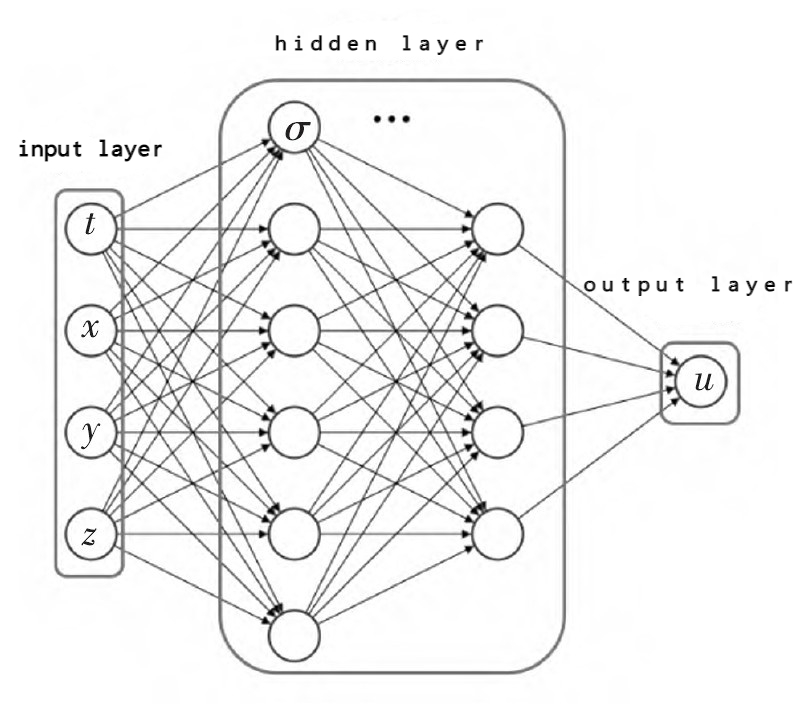
\includegraphics[width=3.5in]{figure/fig1.png}
\caption{邻接矩阵}
\label{fig_1}
\end{figure}

为了理解P-OPT的思想,我们先介绍T-OPT(Transposd-based Cache Replacement)替换策略,T-OPT 可以在不知道未来访问的情况下效仿Belady 的 MIN 策略。存储图可以使用邻接表或邻接矩阵,这里采用的是邻接矩阵,通常,邻接矩阵是稀疏的,如图\ref{fig_1}所示。为了节省存储空间和提高运行效率,可以采用稀疏矩阵的压缩模式:按列压缩(Compressed Sparse Column,CSC),可以快速访问顶点的传入邻居;按行压缩(Compressed Sparse Row,CSR),可以快速访问顶点的传出邻居。

\begin{figure}[!t]
\centering
\includegraphics[width=3.5in]{figure/fig2.png}
\caption{示例算法}
\label{fig_2}
\end{figure}

我们以上图算法为例来讲述T-OPT的替换策略。算法的执行过程是顺序访问每个顶点并处理其所有传入邻居,当缓存被占用满,但需要进行下一次访问时,T-OPT就会执行替换策略,比较缓存行中所有顶点下一次访问的时间,替换距离下一次访问最远的顶点。那么如何查看下一次访问的时间呢?在图\ref{fig_1}当中,处理$D_{0}$的所有传入邻居时,假如访问到了$S_{1}$,通过CSR矩阵可以快速知道下一次访问是在处理D4的传入邻居时,时间复杂度是$O(|Out Degree|)$。但是T-OPT存在着两个局限性:一是运行时间,当缓存行中有多个顶点时,比较所有顶点的下一次访问时间,时间开销会很大。二是会产生缓存竞争,因为缓存中节点的顺序是随机的,当我们使用偏移数组和邻居数组查询邻居时,会导致不规则的内存访问,从而造成缓存竞争。

\begin{figure}[!t]
\centering
\includegraphics[width=3.5in]{figure/fig3.png}
\caption{Rereference Matrix}
\label{fig_3}
\end{figure}

在所以在T-OPT的基础上优化,得到了P-OPT策略。为了提升效率,T-OPT创建了一种新的数据结构,叫做Rereference矩阵,矩阵的每一行是一个缓存行,每一列代表一个时间周期,矩阵的每个元素,代表的是访问节点时的时间周期,与下一次访问该节点所在时间周期之间的距离。比如在$E_{0}$这个时间周期中,$C_{0}$处的值为1,代表下一次访问是在$E_{1}$,$C_{1}$处的值为2,代表下一次访问是在$E_{2}$。
P-OPT突破了T-OPT在运行时间和缓存竞争中的局限性。运行时间方面,P-OPT在Rereference矩阵的每一行存储下一次访问的信息,获取这些信息的代价是$O(1)$。缓存竞争方面,在每个时间周期中,我们只要存储矩阵的一列就足够了,大大减少了缓存竞争。

对多个应用程序和输入的评估表明,P-OPT 提高了图应用程序的缓存局部性,与 LRU 替换相比,平均性能提高了$33\%$(最大$56\%$)。


\subsection{Ripple: Profile-Guided Instruction Cache Replacement for Data Center Applications}

\hspace{0.5em}现代的数据中心应用具有深度的软件堆栈,面临的指令工作集大小比当今处理其支持的指令缓存大小大几个数量级。经常导致指令缓存未命中,使得执行过程出现明显的停顿,因此提出了一种新的缓存替换策略,Ripple\cite{khan2021ripple}。
为了减轻指令缓存未命中的影响,指令缓存未命中缓解机制已经被广泛研究,一些先前的工作提出了分支预测、硬件上的指令预提取器。尽管这些技术很有前景,但它们在现在的处理器上实现,还需要额外的硬件支持,并且未能达到最理想的情况,也就是不会发生指令未命中。

Ripple,是一种新颖的配置文件引导替换技术,可仔细识别导致指令缓存未命中的程序上下文,并努力替换将被理想策略替换的缓存行。Ripple 的操作与底层指令缓存替换策略无关。它会在链接时在适当的程序位置谨慎地注入“缓存行替换”指令,以协助在硬件中实施任意替换策略。 Ripple 不会引入额外的硬件开销,并且可以很容易地在即将发布的处理器上实现。 Ripple 使现有的替换策略能够进一步缩小性能差距以实现理想的 指令缓存替换性能。

\begin{figure}[!t]
\centering
\includegraphics[width=3.5in]{figure/fig4.png}
\caption{Ripple}
\label{fig_4}
\end{figure}

图\ref{fig_4}显示了 Ripple 的设计思路。第一步,在应用运行时,Ripple 使用基于硬件的高效控制流跟踪支持,例如Intel PT或者Last Branch Record,在线分析程序的基础块执行序列。 第二步,使用理想的指令缓存替换策略离线分析程序跟踪以计算一组线索块。线索块是一个基本块,其执行几乎总是导致理想的缓存行被替换。 Ripple策略背后的关键思想是模仿一种理想的策略,该策略将替换未来最长时间不会被访问的缓存行。第三步,在重新编译期间,Ripple 在线索块中注入指令,替换那些缓存行。

我们使用九个流行的数据中心应用程序评估 Ripple,并证明 Ripple 支持任何替换策略来实现更接近理想指令缓存的加速。具体来说,由于平均 $19\%$(最高$28.6\%$)的指令缓存未命中情况减少,Ripple 比之前的工作实现了$1.6\%$(最高$2.13\%$)的平均性能提升。



\subsection{RLR: Designing a Cost-Effective Cache Replacement Policy using Machine Learning}

人们已经进行了广泛的研究来改进缓存替换策略,但设计一种有效的缓存替换策略来降低硬件开销仍然是一项具有挑战性和耗时的任务。鉴于人们对应用机器学习来解决具有挑战性的计算机体系结构设计问题的兴趣激增,我们使用机器学习作为离线工具来设计具有成本效益的缓存替换策略。我们证明机器学习能够指导和加速缓存替换策略的生成,该策略可与最先进的手工策略相媲美。


鉴于行为的影响是符合马尔可夫的,强化学习有可能学习理论上的最优策略。由于强化学习能够适应环境的动态变化并处理所选动作的重要后果,因此非常适合缓存替换问题。我们将缓存替换视为马尔可夫决策过程(Markov Decision Process,MDP),其中代理器(agent)做出替换决策。给定缓存状态,代理器的替换决策将缓存移动到新状态。根据替换决策与 BELADY替换策略的接近程度,分配给代理器一定的奖励,接近程度越高,奖励越高。在我们的框架中,我们使用强化学习算法训练神经网络来学习替换策略。尽管学习到的策略可能是高效的,但由于功率、面积和时序限制,我们不想在硬件中构建神经网络。相反,我们分析神经网络并使用从神经网络中获得的见解来推导一种可以在硬件中实现的替代算法。


\begin{figure}[!t]
\centering
\includegraphics[width=3.5in]{figure/fig5.png}
\caption{Simulation framework overview}
\label{fig_5}
\end{figure}

算法的整体流程图如图\ref{fig_5}所示,
\begin{enumerate}
\item 命中的话,就进行下一次迭代。
\item 未命中的话,cache simulator就会和agent交互,来进行一次缓存置换。
\item 关于未命中的而信息以及命中集合的信息都被通过state vector的方式送给agent。
\item agent会评估state vector并为n路关联缓存生成一个n维的输出向量,其中的每一维向量表示一个cache set的通路,他的值反应其重要性。
\item cache simulator会根据输出向量进行一个置换策略,同时一个反馈会被发送给agent。反馈的评价指标是选择换出的内存在短期内是否会被调用。

\end{enumerate}

下面定义一些特性,并举与这些特性设计了新的策略,能够在硬件中以可接受的开销实现。
\begin{enumerate}
\item 预用距离(preuse distance):我们将预用距离定义为缓存行过去的重用距离。它被计算为缓存行的最后一次访问和当前访问之间的集合访问次数。访问预用和行预用特征都显示出很高的权重。
\item 最新访问类型(Line Last Access Type):缓存行的Last Access type定义为最新的访问类型。预取的缓存行具有最短的缓存生命周期,并且代理器更愿意比其他访问类型的缓存行更早地替换它们。
\item 总调用次数(Line Hits Since Insertion): Hits since insertion告诉我们一个缓存行从被带入缓存后被访问了多少次。代理器倾向于替换命中次数较少的缓存行。在设计缓存替换策略时,我们可以通过保留命中率更高的缓存行来模仿这种行为。
\item 调用频率(Recency):Recency是指一个缓存行在一个集合中的相对访问顺序。 Recency 值的范围从零到(Set Associativity − 1);零表示最近最少使用的缓存行,(Set Associativity − 1) 表示最近使用的缓存行。例如,LRU 替换策略替换最近值为0的缓存行。
\end{enumerate}

在RLR\cite{sethumurugan2021designing}中,重用距离是根据缓存行的预使用距离预测的。年龄小于预测重用距离的缓存行受到保护。此外,缓存行根据其先前访问的类型以及缓存行是否已收到命中来确定优先级。当做出替换决定时,集合中的高速缓存行被分配优先级。优先级是根据缓存行的年龄、以前的访问和命中率计算的。在缓存未命中时,优先级最低的缓存行将被逐出。

几个重要的优先级如下:
\begin{itemize}
\item 年龄优先级(Age priority):每个缓存行都增加了一个年龄计数器,该计数器计算该行在集合访问中的年龄,即自该行的最后一次访问以来该集合被访问了多少次,记为$P_{age}$。
\item 类型优先级(Type priority):每个缓存行都增加了一个类型寄存器,指示其先前的访问是否是预取,记为$P_{type}$。
\item 命中优先级(Hit priority):每个缓存行都增加了一个命中寄存器,该寄存器在缓存行被命中时设置,记为$P_{hit}$。

\end{itemize}

每个缓存行的优先级被计算为上述优先级的加权和,$P_{line} = 8 P_{age} + P_{type} + P_{hit}$。

在这项工作中,我们使用强化学习来学习缓存替换策略。在分析学习到的模型之后,我们能够专注于一些可能影响系统性能的关键特征。使用强化学习提供的见解,我们成功地推导出了一个新的缓存替换策略强化学习替换(Replacment Learned Replacement,RLR)。与最先进的策略相比,RLR具有较低的硬件开销,无需修改处理器的控制和数据路径即可传播程序计数器等信息。平均而言,RLR 比 LRU 将单核和四核系统性能提高了$3.25\%$和$4.86\%$,2MB 末级缓存 (LLC) 的开销为 16.75KB,8MB LLC 的开销为 67KB。


\subsection{GLider: Applying Deep Learning to the Cache Replacement Problem}

尽管深度学习在许多领域都取得了成功,但由于这些模型大且慢,因此不太适合用于硬件预测器。现代微处理器包括许多硬件预测其,用于分支预测、缓存替换、数据提取等,而深度学习提供了一种训练这些预测器的办法,所以可以使用深度学习来帮助设计新的缓存替换策略。对于缓存替换,强大的 LSTM 学习模型可以在离线设置中提供比当前硬件预测器更好的准确性。通过执行分析来解释这个 LSTM 模型,得出一个关键见解,使我们能够设计一个简单的在线模型,该模型与离线模型的准确性相匹配,并且成本降低了几个数量级。

这种替换策略建立在 Hawkeye 缓存替换策略的基础上,该策略将缓存替换描述为一个监督学习问题,其中根据过去缓存访问的最佳缓存解决方案训练预测器。

\begin{figure}[!t]
\centering
\includegraphics[width=3.5in]{figure/fig6.png}
\caption{Overview of the Hawkeye Cache}
\label{fig_6}
\end{figure}


图\ref{fig_6}展示了Hawkeye替换策略的整体结构。它的主要组件是 OPTgen,它模拟最优解的行为以生成训练标签,以及用来学习最优解的Hawkeye预测器。Hawkeye预测器是一个二元分类器,其目标是预测内存访问加载的数据是否有可能被最优算法缓存。缓存友好数据以高优先级插入缓存,缓存厌恶数据以低优先级插入。Hawkeye使用PC作为一项功能并维护一个计数器表,以了解给定PC的内存访问是缓存友好型还是缓存厌恶型。虽然Hawkeye缓存替换策略非常成功,但它的简单预测器在一组具有挑战性的基准测试中仅达到 $72.4\%$ 的准确率。

我们的解决方案提高了Hawkeye的准确性。由于Hawkeye从最优缓存解决方案中学习,因此Hawkeye预测器准确性的改进导致更接近 Belady 最优解决方案的替换决策,从而导致更高的缓存命中率。为了提高预测器的准确性,我们注意到现代替换策略使用有限的程序上下文(PC)来学习重复缓存行为。例如,如果给定 PC 加载的行倾向于缓存友好,那么这些策略将预测同一台PC未来的访问也将缓存友好。我们的工作旨在通过利用更丰富的动态程序上下文来提高预测准确性,特别是导致当前内存访问的过去内存访问序列。因此,我们将缓存替换制定为序列标记问题,其中目标是使用二进制标签标记序列中的每个访问。更具体地说,输入是由他们的PC识别的一系列负载,目标是了解PC是否倾向于访问缓存友好或缓存厌恶的线路。

我们选择通过他们的 PC 而不是他们的内存地址来识别负载有两个原因。首先,PC 的数量较少,因此它们比内存地址重复的频率更高,从而加快了训练速度。其次,更重要的是,LSTM 的大小和学习时间都与唯一输入的数量成正比,并且由于唯一地址的数量比LSTM的典型输入大 100-1000 倍,因此使用内存地址对于 LSTM 是不可行的。

下面介绍用于缓存替换的LSTM模型,模型分为3部分:(1) 无约束离线缓存模型。首先,我们设计了一个离线训练的无约束缓存模型。我们的离线模型使用具有注意机制的 LSTM,该机制可识别输入序列中的重要PC,该模型明显优于最先进的鹰眼预测器。 (2)离线分析。其次,我们分析了注意力层并发现了一个重要的见解:缓存决策主要取决于是否存在少量内存访问,而不是完整的有序序列。因此,我们可以更紧凑地编码我们的输入特征(PC 的历史),以便可以通过简单的硬件友好线性模型在硬件中轻松识别重要的内存访问。 (3) 实用的在线模型。第三,我们使用我们分析的结果来构建一个实用的 SVM 模型,记作ISVM,该模型经过在线训练以识别少数重要的PC,ISVM 模型的精度接近于更大更慢的 LSTM,它的在线版本本质上是一个感知器。

Glider 缓存替换策略由 ISVM 模型和 k-sparse 特征组成\cite{shi2019applying}。我们对来自 SPEC 2006、SPEC 2017 和 GAP(图形处理)基准套件的一组 33 个内存密集型程序进行评估。在单核设置中,Glider 的表现优于第二届缓存替换锦标赛的顶级选手,将 LRU 的未命中率降低了 $8.9\%$,而 Hawkeye 降低了 $7.1\%$,MPPPB 降低了 $6.5\%$,SHiP++ 降低了 $7.5\%$。在四核系统上,Glider 将 IPC 比 LRU 提高了 $14.7\%$,而改进了 $13.6\%$(Hawkeye)、$13.2\%$(MPPPB)和 $11.4\%$(SHiP++)。





\section{Conclusion}

本文讲述了四种缓存替换策略。

\begin{itemize}
\item P-OPT。
P-OPT的主要思想是图的转置简洁地编码了所有图数据的下一个参考信息,从而为图分析工作负载启用了转置驱动的 Belady 的 MIN 替换策略 (T-OPT)。我们介绍了 P-OPT,它是 T-OPT 的一种实际实现,它利用量化来有效地存储和访问下一个参考信息,以做出更好的替换决策。对一系列工作负载和输入图的评估表明,与之前最先进的图分析替换策略和局部优化相比,P-OPT 提供了显着的性能和局部改进。
\item Ripple。
现代数据中心应用程序具有大量指令占用空间,导致大量 I-cache 未命中。尽管许多先前的提议旨在减少 I-cache 未命中,但它们仍然达不到理想的缓存。我们调查了为什么现有的 I-cache 未命中缓解机制实现次优加速,并发现广泛研究的指令预取器会导致浪费的预取引起的驱逐,而现有的替换策略无法缓解。为了实现更智能的驱逐,我们提出了 Ripple,这是一种新颖的配置文件引导的替换技术,它使用程序上下文来告知底层替换策略有关有效替换决策的信息。 Ripple 识别导致 I-cache 未命中的程序上下文,并在链接时在合适的程序位置谨慎地注入“缓存行驱逐”指令。我们使用九个流行的数据中心应用程序评估了 Ripple,并证明它与替换策略无关,即它使任何替换策略都能实现比理想 I-cache 快 $44\%$ 的加速。
\item RLR。
机器学习在架构设计探索中很有用。然而,人类的专业知识对于破译 ML 模型、进行设计权衡和寻找实用的解决方案仍然至关重要。在这项工作中,为了设计一种具有成本效益的缓存替换策略,我们使用强化学习来指导和加快我们的设计。我们使用在 LLC 中相对容易获得的特征来训练 RL 代理。考虑到将 PC 信息传播到 LLC 的复杂性,我们有意将 PC 排除在功能集中之外。在训练代理神经网络后,我们通过分析神经网络权重从大型特征集中识别重要特征。基于从神经网络中得出的见解,我们成功地推导出了一个新的策略以进一步减少硬件开销。总体而言,拟议的更换政策优于 DRRIP(不基于 PC 的政策),并实现了与现有基于 PC 的更换政策相当的性能。



\item Glider。
当我们考虑将机器学习应用于硬件预测问题时,我们通常会关注学习模型。9 例如,作为一种学习模型,感知器优于饱和计数器表,因为感知器可以有效地组合来自多个输入的结果。事实上,这篇论文提出了一种新的缓存替换策略,它使用 SVM(相当于感知器)来超越最先进的技术。然而,Glider 成功的关键不仅仅是使用感知器——我们不是第一个使用感知器来替换缓存的人。相反,正是将适当的特征与感知器结合使用才使其有效。因此,本文展示了我们如何在离线设置中使用深度学习来获得洞察力,从而改进一组特征,从而预测缓存替换。

更广泛地说,我们设计 Glider 的方法表明,深度学习可以在系统地探索特征和特征表示方面发挥重要作用,这些特征和特征表示可以提高更简单模型(例如感知器和 SVM)的有效性。但是,领域知识对于这种方法的工作至关重要。特别是,领域专家必须适当地表述问题,提供相关特征以构建有效的离线模型,并使用间接方法来解释经过训练的模型。我们的论文说明了这种方法成功的一个实例,但我们希望本文中提出的见解和技术能够激发其他微架构预测问题(例如分支预测、数据预取和值预测)的类似解决方案的设计。
\end{itemize}



% An example of a floating figure using the graphicx package.
% Note that \label must occur AFTER (or within) \caption.
% For figures, \caption should occur after the \include.
% Note that IEEEtran v1.7 and later has special internal code that
% is designed to preserve the operation of \label within \caption
% even when the captionsoff option is in effect. However, because
% of issues like this, it may be the safest practice to put all your
% \label just after \caption rather than within \caption{}.
%
% Reminder: the "draftcls" or "draftclsnofoot", not "draft", class
% option should be used if it is desired that the figures are to be
% displayed while in draft mode.
%
%\begin{figure}[!t]
%\centering
%\includegraphics[width=2.5in]{myfigure}
% where an .eps filename suffix will be assumed under latex, 
% and a .pdf suffix will be assumed for pdflatex; or what has been declared
% via \DeclareGraphicsExtensions.
%\caption{Simulation results for the network.}
%\label{fig_sim}
%\end{figure}

% Note that the IEEE typically puts floats only at the top, even when this
% results in a large percentage of a column being occupied by floats.
% However, the Computer Society has been known to put floats at the bottom.


% An example of a double column floating figure using two subfigures.
% (The subfig.sty package must be loaded for this to work.)
% The subfigure \label commands are set within each subfloat command,
% and the \label for the overall figure must come after \caption.
% \hfil is used as a separator to get equal spacing.
% Watch out that the combined width of all the subfigures on a 
% line do not exceed the text width or a line break will occur.
%
%\begin{figure*}[!t]
%\centering
%\subfloat[Case I]{\includegraphics[width=2.5in]{box}%
%\label{fig_first_case}}
%\hfil
%\subfloat[Case II]{\includegraphics[width=2.5in]{box}%
%\label{fig_second_case}}
%\caption{Simulation results for the network.}
%\label{fig_sim}
%\end{figure*}
%
% Note that often IEEE papers with subfigures do not employ subfigure
% captions (using the optional argument to \subfloat[]), but instead will
% reference/describe all of them (a), (b), etc., within the main caption.
% Be aware that for subfig.sty to generate the (a), (b), etc., subfigure
% labels, the optional argument to \subfloat must be present. If a
% subcaption is not desired, just leave its contents blank,
% e.g., \subfloat[].


% An example of a floating table. Note that, for IEEE style tables, the
% \caption command should come BEFORE the table and, given that table
% captions serve much like titles, are usually capitalized except for words
% such as a, an, and, as, at, but, by, for, in, nor, of, on, or, the, to
% and up, which are usually not capitalized unless they are the first or
% last word of the caption. Table text will default to \footnotesize as
% the IEEE normally uses this smaller font for tables.
% The \label must come after \caption as always.
%
%\begin{table}[!t]
%% increase table row spacing, adjust to taste
%\renewcommand{\arraystretch}{1.3}
% if using array.sty, it might be a good idea to tweak the value of
% \extrarowheight as needed to properly center the text within the cells
%\caption{An Example of a Table}
%\label{table_example}
%\centering
%% Some packages, such as MDW tools, offer better commands for making tables
%% than the plain LaTeX2e tabular which is used here.
%\begin{tabular}{|c||c|}
%\hline
%One & Two\\
%\hline
%Three & Four\\
%\hline
%\end{tabular}
%\end{table}


% Note that the IEEE does not put floats in the very first column
% - or typically anywhere on the first page for that matter. Also,
% in-text middle ("here") positioning is typically not used, but it
% is allowed and encouraged for Computer Society conferences (but
% not Computer Society journals). Most IEEE journals/conferences use
% top floats exclusively. 
% Note that, LaTeX2e, unlike IEEE journals/conferences, places
% footnotes above bottom floats. This can be corrected via the
% \fnbelowfloat command of the stfloats package.







% if have a single appendix:
%\appendix[Proof of the Zonklar Equations]
% or
%\appendix  % for no appendix heading
% do not use \section anymore after \appendix, only \section*
% is possibly needed

% use appendices with more than one appendix
% then use \section to start each appendix
% you must declare a \section before using any
% \subsection or using \label (\appendices by itself
% starts a section numbered zero.)
%




% Can use something like this to put references on a page
% by themselves when using endfloat and the captionsoff option.
\ifCLASSOPTIONcaptionsoff
  \newpage
\fi



% trigger a \newpage just before the given reference
% number - used to balance the columns on the last page
% adjust value as needed - may need to be readjusted if
% the document is modified later
%\IEEEtriggeratref{8}
% The "triggered" command can be changed if desired:
%\IEEEtriggercmd{\enlargethispage{-5in}}

% references section

% can use a bibliography generated by BibTeX as a .bbl file
% BibTeX documentation can be easily obtained at:
% http://mirror.ctan.org/biblio/bibtex/contrib/doc/
% The IEEEtran BibTeX style support page is at:
% http://www.michaelshell.org/tex/ieeetran/bibtex/
%\bibliographystyle{IEEEtran}
% argument is your BibTeX string definitions and bibliography database(s)
%\bibliography{IEEEabrv,../bib/paper}
%
% <OR> manually copy in the resultant .bbl file
% set second argument of \begin to the number of references
% (used to reserve space for the reference number labels box)
\begin{thebibliography}{10}


\bibitem{belady1966}
L.~A. Belady, ``A study of replacement algorithms for a virtual-storage
  computer,'' \emph{IBM Systems journal}, vol.~5, no.~2, pp. 78--101, 1966.

\bibitem{karedla1994}
R.~Karedla, J.~S. Love, and B.~G. Wherry, ``Caching strategies to improve disk
  system performance,'' \emph{Computer}, vol.~27, no.~3, pp. 38--46, 1994.

\bibitem{o1993}
E.~J. O'neil, P.~E. O'neil, and G.~Weikum, ``The lru-k page replacement
  algorithm for database disk buffering,'' \emph{Acm Sigmod Record}, vol.~22,
  no.~2, pp. 297--306, 1993.

\bibitem{jain2016back}
A.~Jain and C.~Lin, ``Back to the future: Leveraging belady's algorithm for
  improved cache replacement,'' in \emph{2016 ACM/IEEE 43rd Annual
  International Symposium on Computer Architecture (ISCA)}.\hskip 1em plus
  0.5em minus 0.4em\relax IEEE, 2016, pp. 78--89.

\bibitem{khan2021ripple}
T.~A. Khan, D.~Zhang, A.~Sriraman, J.~Devietti, G.~Pokam, H.~Litz, and
  B.~Kasikci, ``Ripple: Profile-guided instruction cache replacement for data
  center applications,'' in \emph{2021 ACM/IEEE 48th Annual International
  Symposium on Computer Architecture (ISCA)}.\hskip 1em plus 0.5em minus
  0.4em\relax IEEE, 2021, pp. 734--747.

\bibitem{balaji2021p}
V.~Balaji, N.~Crago, A.~Jaleel, and B.~Lucia, ``P-opt: Practical optimal cache
  replacement for graph analytics,'' in \emph{2021 IEEE International Symposium
  on High-Performance Computer Architecture (HPCA)}.\hskip 1em plus 0.5em minus
  0.4em\relax IEEE, 2021, pp. 668--681.

\bibitem{sethumurugan2021designing}
S.~Sethumurugan, J.~Yin, and J.~Sartori, ``Designing a cost-effective cache
  replacement policy using machine learning,'' in \emph{2021 IEEE International
  Symposium on High-Performance Computer Architecture (HPCA)}.\hskip 1em plus
  0.5em minus 0.4em\relax IEEE, 2021, pp. 291--303.

\bibitem{shi2019applying}
Z.~Shi, X.~Huang, A.~Jain, and C.~Lin, ``Applying deep learning to the cache
  replacement problem,'' in \emph{Proceedings of the 52nd Annual IEEE/ACM
  International Symposium on Microarchitecture}, 2019, pp. 413--425.

\bibitem{wu2011ship}
C.-J. Wu, A.~Jaleel, W.~Hasenplaugh, M.~Martonosi, S.~C. Steely~Jr, and
  J.~Emer, ``Ship: Signature-based hit predictor for high performance
  caching,'' in \emph{Proceedings of the 44th Annual IEEE/ACM International
  Symposium on Microarchitecture}, 2011, pp. 430--441.

\bibitem{beckmann2017maximizing}
N.~Beckmann and D.~Sanchez, ``Maximizing cache performance under uncertainty,''
  in \emph{2017 IEEE International Symposium on High Performance Computer
  Architecture (HPCA)}.\hskip 1em plus 0.5em minus 0.4em\relax IEEE, 2017, pp.
  109--120.

\end{thebibliography}

% biography section
% 
% If you have an EPS/PDF photo (graphicx package needed) extra braces are
% needed around the contents of the optional argument to biography to prevent
% the LaTeX parser from getting confused when it sees the complicated
% \includegraphics command within an optional argument. (You could create
% your own custom macro containing the \includegraphics command to make things
% simpler here.)
%\begin{IEEEbiography}[{\includegraphics[width=1in,height=1.25in,clip,keepaspectratio]{mshell}}]{Michael Shell}
% or if you just want to reserve a space for a photo:

%\begin{IEEEbiography}{Michael Shell}
%Biography text here.
%\end{IEEEbiography}

% if you will not have a photo at all:
%\begin{IEEEbiographynophoto}{John Doe}
%Biography text here.
%\end{IEEEbiographynophoto}

% insert where needed to balance the two columns on the last page with
% biographies
%\newpage
%
%\begin{IEEEbiographynophoto}{Jane Doe}
%Biography text here.
%\end{IEEEbiographynophoto}

% You can push biographies down or up by placing
% a \vfill before or after them. The appropriate
% use of \vfill depends on what kind of text is
% on the last page and whether or not the columns
% are being equalized.

%\vfill

% Can be used to pull up biographies so that the bottom of the last one
% is flush with the other column.
%\enlargethispage{-5in}



% that's all folks
\end{document}


